%Created by Roland Pastorino in 2013
%Contact info: roland.pastorino@mech.kuleuven.be / www.rolandpastorino.com
%If you want to include your modifications in the template and make them available for everybody, you can contact the "KU Leuven, Dienst Communicatie, Afdeling Positionering en Marketing" (marketing@dcom.kuleuven.be) or myself.

\documentclass[11pt,t]{beamer}
\mode<presentation> {\usetheme{kuleuven}}

%%%%%%%%%%%%%%%%%%%%%%%%%%%%%%%%%%%%%%%%
%info
\title{Newton-type operator splitting }
\author{Willem Melis}
\institute{KU Leuven}
\subtitle{for embedded model predictive control }
\date{september 13, 2017, Leuven, Belgium}
%pdf metadata
	\subject{Newton-type operator splitting for embedded model predictive control}
	\keywords{Newton-type operator splitting,  model predictive control, embedded}
\graphicspath{{graphics/}} % path to the graphics folder

\usepackage{amsmath}
\DeclareMathOperator{\project}{project}
\DeclareMathOperator{\prox}{prox}
\DeclareMathOperator*{\minimize}{minimize}
\DeclareMathOperator*{\argmin}{arg\,min}

%%%%%%%%%%%%%%%%%%%%%%%%%%%%%%%%%%%%%%%%
\begin{document}
%title page
	\setbeamertemplate{headline}[title_page]
	\setbeamertemplate{footline}[title_page]
	\csname beamer@calculateheadfoot\endcsname %recalculate head and foot dimension
		\begin{frame}
			\titlepage
		\end{frame}
%head and foot for body text	
	\setbeamertemplate{headline}[body]
	\setbeamertemplate{footline}[body]


%%%%%%%%%%%%%%%%%%%%%%%%%%%%%%%%%%%%%%%%%%
\begin{frame}{Outline}
	\vskip 5mm
	\hfill	{\large \parbox{.95\textwidth}{\tableofcontents[hideallsubsections]}}
\end{frame}
\section{Introduction}
\begin{frame}{Introduction: What is the goal?}
\begin{itemize}
	\item Easy to use (for control engineers) software that generates a NMPC controllers
	\item User defines conditions ,system behavior and some NMPC options.
	\item Program generates NMPC controller e.g. optimalInputs=NMPC(currentStates)
	\item Aimed at embedded devices (different platforms)
	\item Using only C89 standard
	\item Low memory usage
\end{itemize}
\end{frame}

\section{PANOC}
\begin{frame}{Projected gradient descent}
\begin{equation}
x^k = x^{k-1} - \gamma \nabla f(x^{k-1})
\label{eq:grad descent}
\end{equation}

\begin{equation}
x^k = \project_{A}[ x^{k-1} - \gamma \nabla f(x^{k-1})]
\label{eq:projected grad descent}
\end{equation}

\end{frame}
%--------------------------------------
\begin{frame}{Forward backward splitting}
	
	\begin{itemize}
		\item Solve the problem $ \minimize\quad f(x) + g(x)$
		
		\begin{equation}
		x^k = \prox_{g}\big( x^{(k-1)}- \gamma \nabla f(x^{(k-1)})\big)
		\label{eq:prox grad method}
		\end{equation}
		\begin{equation}
		\prox_g(x)=\argmin_u(g(u) + \frac{1}{2}||u-x||^2_2)
		\end{equation}
		\begin{equation}
		I_A = 
		\begin{cases}
		0 & x \in A  \\
		\infty & x \notin A
		\end{cases}
		\label{eq:indicator function}
		\end{equation}
		\item Speedup convergence?
	\end{itemize}	
\end{frame}

\begin{frame}{speedup FBS}
	\begin{itemize}
		\item Fixed point equation $x^{k+1}=F(x^k)$
		\item Residue
			\begin{equation}
				R = x^k - F(x^k)
			\end{equation}
			\begin{equation}
			R_{\gamma}(u)= \frac{1}{\gamma}\left[ u - prox_g( u - \nabla f(u)\gamma) \right]
			\label{eq:residue prox grad method}
			\end{equation}
			
			\begin{equation}
			u^{k+1} = u^k -H_kR_{\gamma}(u^k)
			\label{eq:newton iteration FBS}
			\end{equation}
		\item Incorporate curvature information in the algorithm
		\item Solve with lbgfs
	\end{itemize}
\end{frame}

\begin{frame}{speedup FBS}
\begin{itemize}
	\item FBE: forward backward envelop
	\begin{equation}
	\varphi_{\gamma} = f(x) - \frac{\gamma}{2}||\nabla f(x)||^2 + g^{\gamma} \big(x-\gamma \nabla f(x) \big)
	\label{eq:smoothed opti problem}
	\end{equation}
	\begin{equation}
	u^{k+1} = u^k - (1-\tau_k)\gamma r^k + \tau_kd^k
	\label{eq:PANOC convex combination}
	\end{equation}
	\item If not used, only fast convergence if close enough too solution or worse might diverge
	\item Globalization technique
	
\end{itemize}
\end{frame}

\section{NMPC}
%--------------------------------------
\begin{frame}{Nonlinear model predictive control (NMPC)}
	\begin{itemize}
		\item Finite-horizon optimal control problem
		
		\begin{equation}
		\begin{aligned}
		& \underset{u}{\text{min}}	&& \sum_{n=0}^{N-1}l_n(x_n,u_n) + g_n(u_n) + l_N(x_N) \\
		& \text{subject to}			&& x_0 = \bar{x} \\
		& 							&&  x_{n+1} = f_n(x_n,u_n), n=0...N-1
		\end{aligned}
		\end{equation}
		\item Single shoot
		\item Multiple shooting
		\item Discretization
		\item Gradient ?
	\end{itemize}
\end{frame}

\begin{frame}{Casadi}
	\centering
	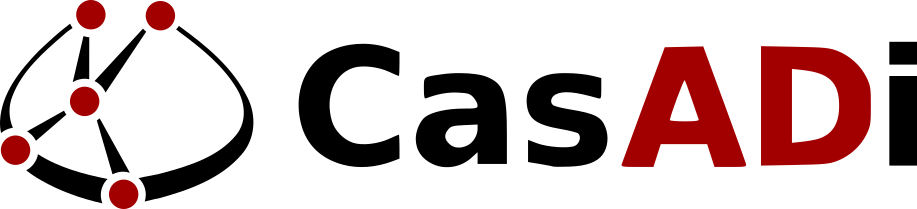
\includegraphics[width=5cm, height=2cm]{casadi.png}
	\begin{itemize}
		\item Symbolic framework
		\item Automatic differentiation
		\item Discretization(if needed)
		\item Code generation
	\end{itemize}
\end{frame}

\section{Implementation}
\begin{frame}{Overview Code}
\begin{figure}
	\centering
	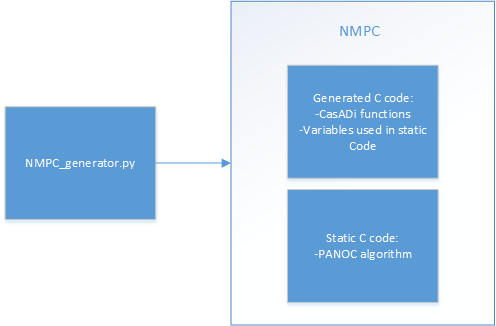
\includegraphics[width=10cm, height=7cm]{DrawingVisio.png}
\end{figure}
\end{frame}

\begin{frame}{Questions}
\begin{itemize}
	\item https://github.com/kul-forbes/nmpc-codegen
\end{itemize}
\end{frame}

\end{document}